\chapter{Boosted Higgs at the LHC} \label{chap:higgs}

In \cref{chap:standard_model} I've shown how the higgs mechanism resolves
inconsistencies of the model surrounding the generation of gauge boson and
fermion mass terms while also maintaining gauge invariance.  However to
understand the search for and resulting discovery of this SM Higgs boson
requires the discussion of how one goes about producing and detecting the
physical object itself.  In order to gather sufficient statistics to validate
the theory we require a collider capable of putting enough energy into a
collision to rapidly produce Higgs bosons for study.  To this end the Large
Hadron Collider (LHC) discussed in \cref{chap:lhc} was laboriously
designed, funded, and constructed by the largest international collaboration of
scientists on the planet. In this chapter I will discuss the relevant Higgs
boson production mechanisms available at the LHC as well as the various decay
modes of the Higgs that were used for its discovery, and are currently used to
measure its properties.

\section{Higgs Production Mechanisms} \label{sec:higgs:production}

At the LHC the dominant production mechanisms for the Higgs boson in order of
decreasing cross section are: gluon-fluon fusion (ggF), vector boson fusion
(VBF), vector boson associated production or ``Higgsstrahlung" (VH), and
associated production with $t\bar{t}$ ($t\bar{t}H$) and $b\bar{b}$
($b\bar{b}H$).  The cross sections for the signatures of these processes with
associated theoretical uncertainties for each are shown as a function of the
center-of-mass energy $\sqrt{s}$ in \Cref{fig:higgs_xsection}, and the
leading order (LO) Feynman diagrams can be seen in \Cref{fig:higgs_production}.

\begin{figure}[!htbp]
  \begin{center}
    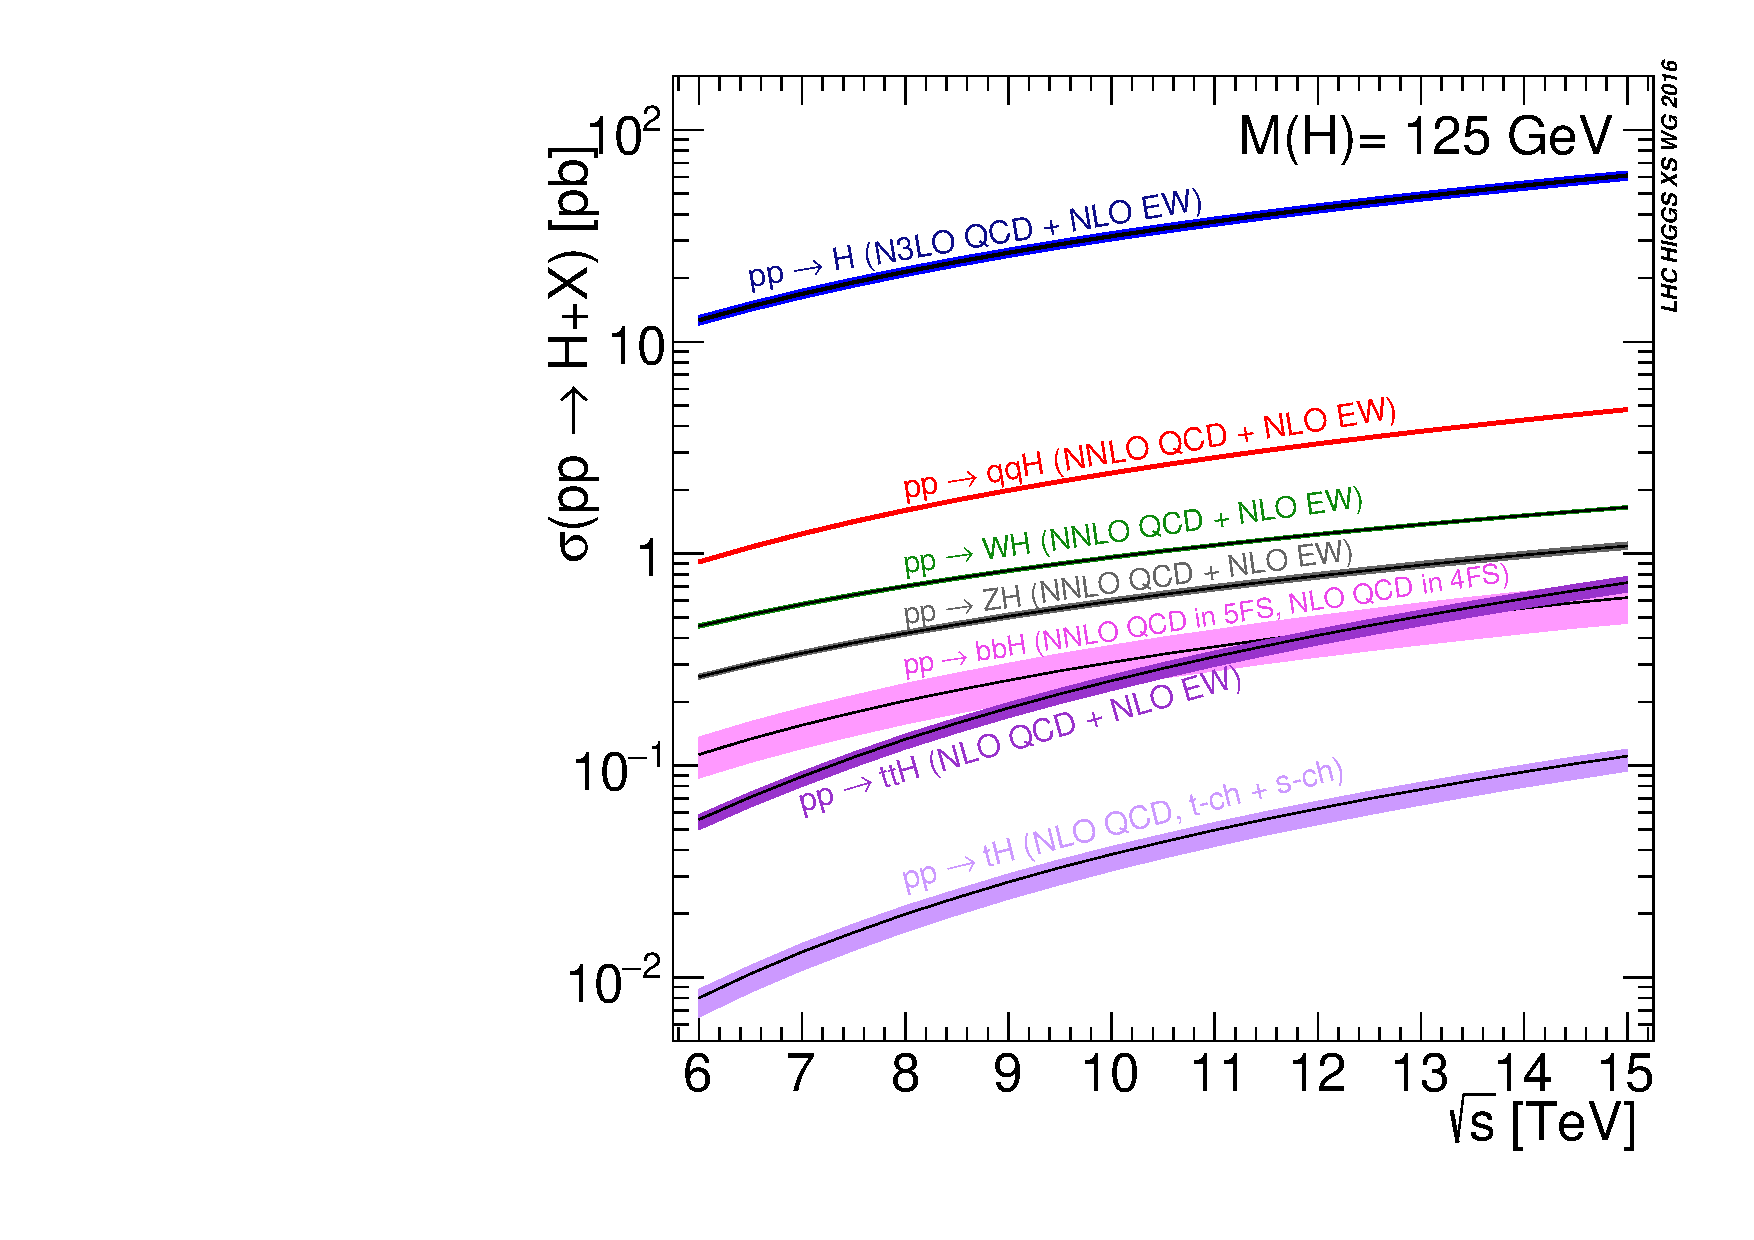
\includegraphics[width=0.5\linewidth]{figures/higgs/higgs_xsection.pdf}
    \caption{Cross sections for the production of the SM Higgs boson signatures
as a function of the center of mass energy ($\sqrt{s}$) at the LHC
\cite{PDG2018:Ch11}.  In order of decreasing cross section: the ggF process
signature is $H$, the VBF process signature is $qqH$, the VH process signature
is split into $WH$ and $ZH$, and the $b\bar{b}$ / $t\bar{t}$ signatures are
$t\bar{t}H$ / $b\bar{b}H$.}
    \label{fig:higgs_xsection}
  \end{center}
\end{figure}

The LO Feynman diagram contains the least number of vertices, and thus coupling
constants, making it the largest contribution to the cross section calculation.
Adding an additional vertex, represents a higher order correction to the LO
calculation known as next-to-leading order (NLO) where each additional vertex
adds a ``next" (NNLO, N3LO, etc.). For reference, the current best
estimates of the production cross sections for the leading production
mechanisms are detailed in \Cref{table:higgs_production_xsection}.

\begin{figure}[!htbp]
\centering

\subcaptionbox{gluon-gluon fusion}{
\resizebox{0.48\textwidth}{!}{
\begin{tikzpicture}[thick]
 \begin{feynman}
  \vertex (origin);
  \vertex [right=1.5cm of origin] (H);
  \vertex [above left=1cm and 1.2cm of origin] (v1);
  \vertex [below left=1cm and 1.2cm of origin] (v2);
  \vertex [left=1.75cm of v1] (g1) {\(g\)};
  \vertex [left=1.75cm of v2] (g2) {\(g\)};
  \diagram* {
  (origin) -- [red, scalar, edge label={\(H\)}] (H),
  (origin) -- [fermion] (v1) -- [fermion] (v2) -- [fermion] (origin),
  (g1) -- [gluon] (v1),
  (g2) -- [gluon] (v2),
  };
 \end{feynman}
\end{tikzpicture}
}}
\subcaptionbox{vector boson fusion}{
\resizebox{0.48\textwidth}{!}{
\begin{tikzpicture}[thick]
 \begin{feynman}
  \vertex (origin);
  \vertex [right=1.5cm of origin] (H);
  \vertex [above left=1cm and 1.2cm of origin] (v1);
  \vertex [below left=1cm and 1.2cm of origin] (v2);
  \vertex [left=1.75cm of v1] (q1) {\(q\)};
  \vertex [left=1.75cm of v2] (q2) {\(q\)};
  \vertex [above right=0.25cm and 1.75cm of v1] (q3) {\(q'\)};
  \vertex [below right=0.25cm and 1.75cm of v2] (q4) {\(q'\)};
  \diagram* {
  (v1) -- [boson, edge label={\(V\)}] (origin),
  (origin) -- [boson, edge label={\(V\)}] (v2),
  (origin) -- [red, scalar, edge label={\(H\)}] (H),
  (q1) -- [fermion] (v1),
  (q2) -- [fermion] (v2),
  (v1) -- [fermion] (q3),
  (v2) -- [fermion] (q4),
  };
 \end{feynman}
\end{tikzpicture}
}} \\
\subcaptionbox{associated production}{
\resizebox{0.48\textwidth}{!}{
\begin{tikzpicture}[thick]
 \begin{feynman}
  \vertex (origin);
  \vertex [right=1.2cm of origin] (Vstar);
  \vertex [above right=0.50cm and 1.0cm of Vstar] (V1) {\(V\)};
  \vertex [red, below right=0.50cm and 1.0cm of Vstar] (H) {\(H\)};
  \vertex [above left=0.50cm and 1.0cm of origin] (g1) {\(\bar{q}\)};
  \vertex [below left=0.50cm and 1.0cm of origin] (g2) {\(q\)};
  \diagram* {
  (origin) -- [boson, edge label={\(V^{*}\)}] (Vstar) -- [boson] (V1),
  (Vstar) -- [red, scalar] (H),
  (origin) -- [fermion] (g1),
  (g2) -- [fermion] (origin),
  };
 \end{feynman}
\end{tikzpicture}
}}
\subcaptionbox{$t\bar{t}$ ($t\bar{t}H$) and $b\bar{b}$ ($b\bar{b}H$)}{
\resizebox{0.48\textwidth}{!}{
\begin{tikzpicture}[thick]
 \begin{feynman}
  \vertex (origin);
  \vertex [right=1.5cm of origin] (H);
  \vertex [above left=1cm and 0.2cm of origin] (v1);
  \vertex [below left=1cm and 0.2cm of origin] (v2);
  \vertex [left=1.75cm of v1] (g1) {\(g\)};
  \vertex [left=1.75cm of v2] (g2) {\(g\)};
  \vertex [above right=1.2cm and 1.4cm of origin] (t1) {\(t,b\)};
  \vertex [below right=1.2cm and 1.4cm of origin] (t2) {\(\bar{t},\bar{b}\)};
  \diagram* {
  (g1) -- [gluon] (v1),
  (g2) -- [gluon] (v2),
  (origin) -- [red, scalar, edge label={\(H\)}] (H),
  (origin) -- [fermion] (v1) -- [fermion] (t1),
  (t2) -- [fermion] (v2) -- [fermion] (origin),
  };
 \end{feynman}
\end{tikzpicture}
}}

\caption{Feynman diagrams representing the dominant Higgs production modes at
the LHC.}

\label{fig:higgs_production}
\end{figure}

\begin{table}[htpb]
 \centering
 \caption{ SM Higgs boson production cross sections in units of pb for
$m_{H}=125~\GeV$ in $pp$ collisions for the current LHC center-of-mass energy,
$\sqrt{s} = 13~\TeV$.  The predictions for the ggF channel include the latest
N3LO results, which have reduced theoretical uncertainties by a factor around 2
compared to the NNLO results \cite{PDG2018:Ch11}.}
 \begin{tabular}{@{}rrrrrrrr@{}} \toprule
  $\sqrt{s}~(\TeV)$ & ggF                  & VBF                  & $WH$                 & $ZH$                 & $t\bar{t}H$            & Total~(pb) \\ \midrule
  $13$              & $48.6_{-5\%}^{+5\%}$ & $3.78_{-2\%}^{+2\%}$ & $1.37_{-2\%}^{+2\%}$ & $0.88_{-5\%}^{+5\%}$ & $0.50_{-13\%}^{+9\%}$ &  $55.1$    \\
  \bottomrule
 \end{tabular}\label{table:higgs_production_xsection}
\end{table}

The dominant Higgs production mechanism at hadron colliders is gluon-gluon
fusion.  This may seem strange as gluons are massless and thus do not couple
directly to the Higgs boson.  Instead the gluons indirectly couple to the Higgs
boson via a quark loop.  As discussed in \Cref{sec:theory:fermion_mass}, the
coupling of a fermion is proportional to $m_f$, so the dominant contribution to
this quark loop comes from the top quark. It is important to note that the ggF
cross section in \Cref{table:higgs_production_xsection} is inclusive in number
of final state jets and thus will include diagrams like the one shown in
\Cref{fig:h_plus_j}.  There has been considerable effort to calculate exclusive
$H$ + jet(s) production process at NLO and NNLO \cite{deFlorian:2016spz} for
use in analysis where there is an explicit requirement for an associated jet
such as the one presented in this dissertation in \Cref{part:HbbISR}.

\begin{figure}[!htbp]
\centering
\begin{tikzpicture}[thick]
 \begin{feynman}
  \vertex (origin);
  \vertex [right=1.5cm of origin] (H);
  \vertex [above left=1cm and 1.2cm of origin] (v1);
  \vertex [below left=1cm and 1.2cm of origin] (v2);
  \vertex [left=1.75cm of v1] (g1) {\(g\)};
  \vertex [left=1.75cm of v2] (g2) {\(g\)};
  \vertex at ($(g1)!0.5!(v1)$) (ISR_start);
  \vertex [above right=0.8cm and 1.5 cm of ISR_start] (ISR) {\(g\)};
  \diagram* {
  (origin) -- [red, scalar, edge label={\(H\)}] (H),
  (origin) -- [fermion] (v1) -- [fermion] (v2) -- [fermion] (origin),
  (g1) -- [gluon] (v1),
  (g2) -- [gluon] (v2),
  (ISR_start) -- [gluon] (ISR),
  };
 \end{feynman}
\end{tikzpicture}
\caption{Feynman diagram for ggF Higgs + jet production.}
\label{fig:h_plus_j}
\end{figure}

The second-largest cross section for Higgs production at the LHC comes from the VBF
mechanism.  In VBF the initial state quarks scatter via the exchange of a
$W^{\pm}$ or $Z$ boson which subsequently radiates the Higgs boson.  Unlike ggF
this production mechanism scatters the initial state quarks which allows them to
be observed as part of the interaction.  The presence of these extra quarks
makes these interactions easier to select during analysis.

The third-largest cross section for Higgs production is in association with a
vector boson. The cross section for this is even smaller than the above two, but
remains important due to the easily selected signature of the decaying vector
boson.  The largest background at the LHC is multijet events coming from
interactions that produce strong force objects.  Thus the leptons from the
boson's decay act as a discriminator against this multijet background, greatly
reducing its effect on sensitivity. Note that the $W/Z$ can also decay
hadronically giving a final state that looks like $H$ + jet.

The lowest cross section of the four methods discussed is the
production of the Higgs boson in association with either $b\bar{b}$ or
$t\bar{t}$.  This channel is important because it allows direct measurement of
the $ttH$ coupling, unlike the ggF method where the quark in the loop is never
directly observed.

\section{Parton Distribution Function} \label{sec:higgs:partons}

The LHC collides protons, however looking at the feynman diagrams in
\Cref{fig:higgs_production} we see that it is quarks and gluons (a.k.a partons)
that produce these fundamental interactions. This is an indicator that when we
calculate the production cross section for a process at the LHC, we have to not
only consider the hard-scatter probability of the specific diagram, but also
consider the composition of the proton itself.  Specifically, we must consider
the fraction of the total momentum of the proton held by each of its constituent
partons.  This concept is described by Parton Distribution Functions (PDFs)
which give the probability that the indicated parton carries momentum fraction
$x$ of the proton when probed at with energy scale $Q$.  An example PDF for $Q =
10\text{GeV}^2$ and $Q = 10^{4}$GeV in \Cref{fig:parton_distribution_function}

\begin{figure}[!htbp]
  \begin{center}
    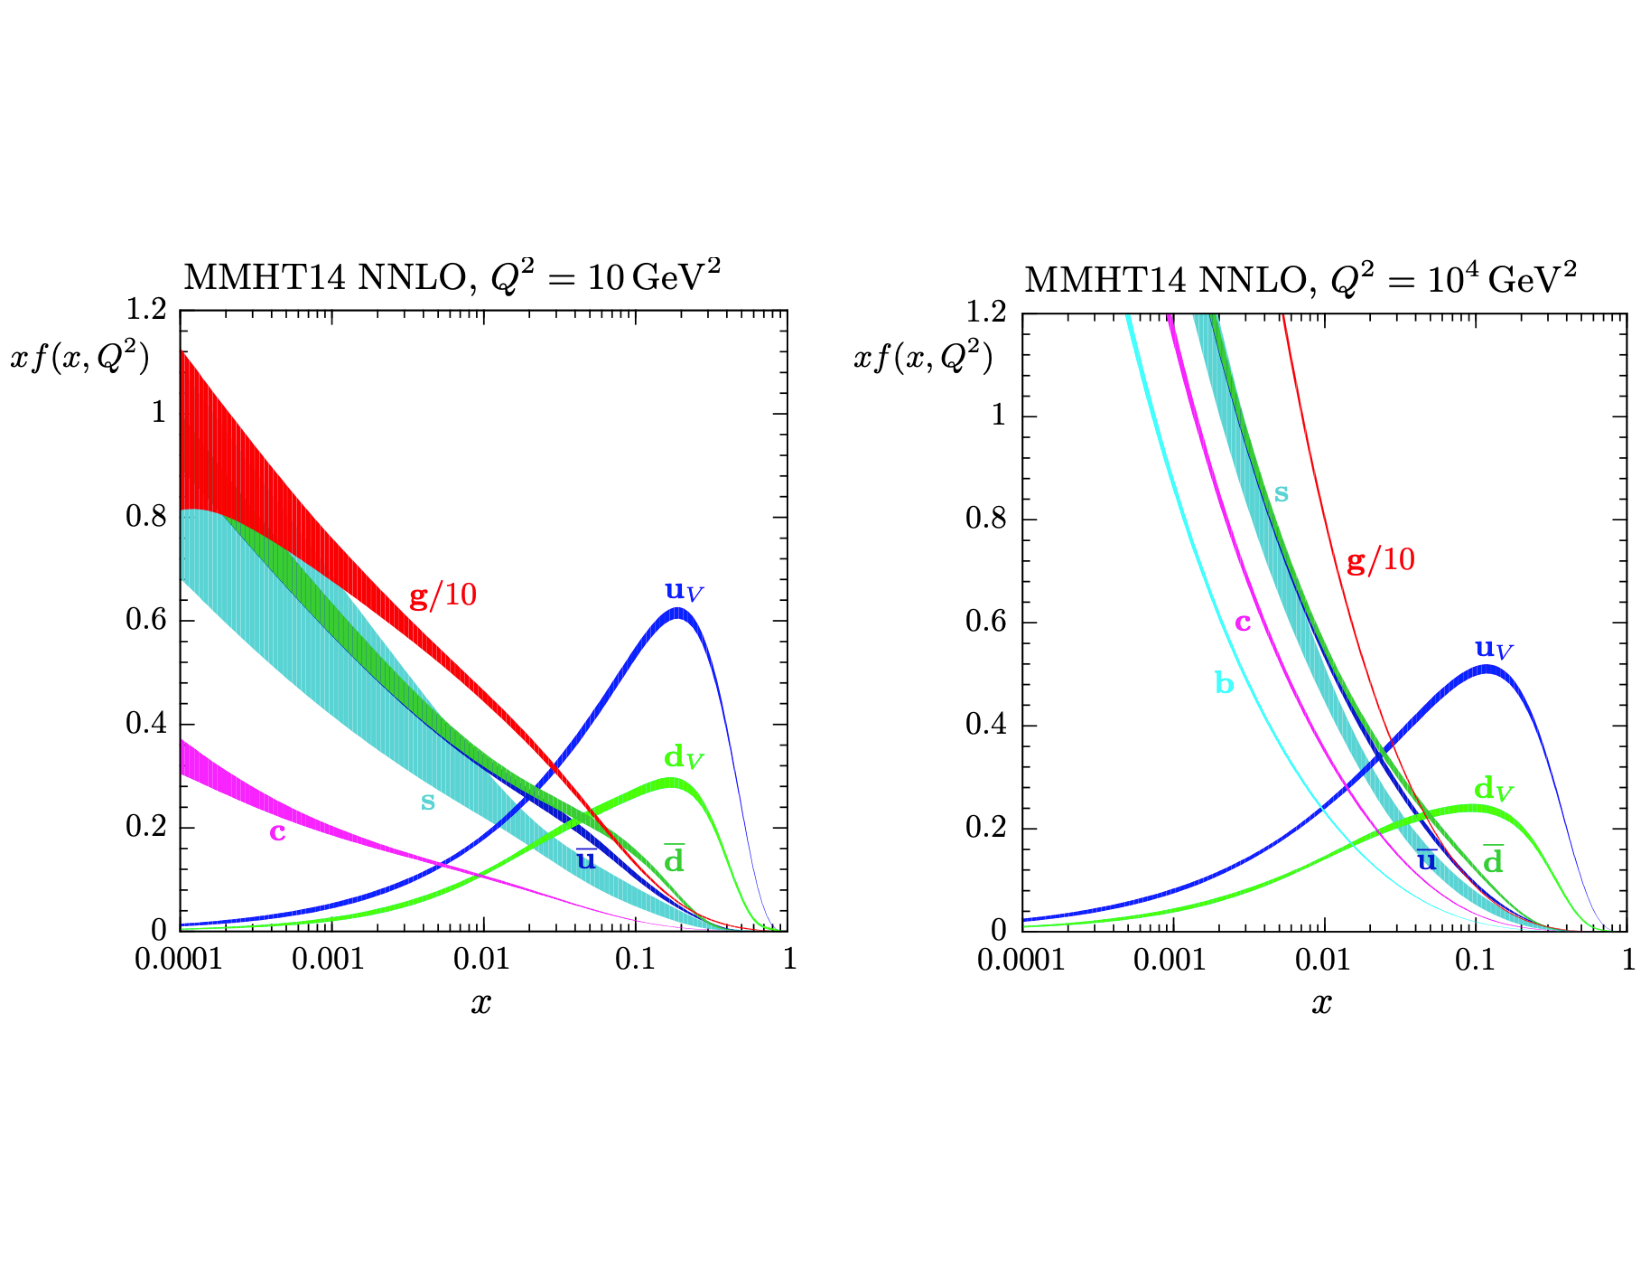
\includegraphics[width=0.8\linewidth]{figures/higgs/pdf.pdf}
    \caption{ \cite{Harland-Lang2015} MMHT2014 NNLO PDFs at $Q2 = 10\text{GeV}^{2}$ and $Q2
=10^{4}\text{GeV}^{2}$ with associated 68\% confidence-level uncertainty bands.
The colored regions indicate the probability of finding the labeled parton with
a momentum fraction given along the x axis. As expected the $u_V$ and $d_V$
contain the largest fraction of the momentum, however we can also see that many
gluons will exist with smaller fractions of the total momentum. Note that as
$Q^2$ increases you are more likely to find something besides a $u/d$}
    \label{fig:parton_distribution_function}
  \end{center}
\end{figure}

\section{Branching Ratios} \label{sec:higgs:branching}

The coupling of the SM Higgs with the gauge bosons and fermions has been shown
to give these particles their mass, however it also means that the Higgs can
decay into all of these particles.  In order of most to least likely final
states of a Higgs decay we have the decay to; a pair of $b$-quarks ($b\bar{b}$),
a pair of weak vector bosons where one is off-shell ($VV^{*}$), two gluons
($gg$), a duo of tau leptons ($\tau^{+}\tau^{-}$), or a pair of photons
($\gamma\gamma$).  Similar to the ggF production mechanism discussed in
\Cref{sec:higgs:production} the decays to massless gauge bosons (photons and
gluons) are facilitated through loops of massive particles. The exact feynman
diagrams depicting the above process' are shown in \Cref{fig:higgs_decay} while
information about their branching ratios is detailed in
\Cref{table:higgs_branching_ratios}.

\begin{figure}[!htbp]
\centering

\subcaptionbox{$H \rightarrow b\bar{b}$}{
\resizebox{0.48\textwidth}{!}{
\begin{tikzpicture}[thick]
 \begin{feynman}
  \vertex (origin);
  \vertex [right=1.5cm of origin] (H);
  \vertex [above right=0.50cm and 1.5cm of H] (b1) {\(\bar{b}\)};
  \vertex [below right=0.50cm and 1.5cm of H] (b2) {\(b\)};
  \diagram* {
  (origin) -- [red, scalar, edge label={\(H\)}] (H),
  (b1) -- [fermion] (H) -- [fermion] (b2),
  };
 \end{feynman}
\end{tikzpicture}
}}
\subcaptionbox{$H \rightarrow W^{\pm}W^{\mp*}$}{
\resizebox{0.48\textwidth}{!}{
\begin{tikzpicture}[thick]
 \begin{feynman}
  \vertex (origin);
  \vertex [right=1.5cm of origin] (H);
  \vertex [above right=0.50cm and 1.5cm of H] (W1) {\(W^{\pm}\)};
  \vertex [below right=0.50cm and 1.5cm of H] (W2) {\({W^{\mp}}^{*}\)};
  \diagram* {
  (origin) -- [red, scalar, edge label={\(H\)}] (H),
  (W1) -- [boson] (H),
  (W2) -- [boson] (H),
  };
 \end{feynman}
\end{tikzpicture}
}} \\
\subcaptionbox{$H \rightarrow gg$}{
\resizebox{0.48\textwidth}{!}{
\begin{tikzpicture}[thick]
 \begin{feynman}
  \vertex (origin);
  \vertex [right=1.5cm of origin] (H);
  \vertex [above right=1cm and 1.2cm of H] (v1);
  \vertex [below right=1cm and 1.2cm of H] (v2);
  \vertex [right=1.75cm of v1] (g1) {\(g\)};
  \vertex [right=1.75cm of v2] (g2) {\(g\)};
  \diagram* {
  (origin) -- [red, scalar, edge label={\(H\)}] (H),
  (H) -- [fermion] (v1) -- [fermion] (v2) -- [fermion] (H),
  (g1) -- [gluon] (v1),
  (g2) -- [gluon] (v2),
  };
 \end{feynman}
\end{tikzpicture}
}}
\subcaptionbox{$H \rightarrow \tau^{+}\tau{-}$}{
\resizebox{0.48\textwidth}{!}{
\begin{tikzpicture}[thick]
 \begin{feynman}
  \vertex (origin);
  \vertex [right=1.5cm of origin] (H);
  \vertex [above right=0.50cm and 1.5cm of H] (tau1) {\(\tau^{+}\)};
  \vertex [below right=0.50cm and 1.5cm of H] (tau2) {\(\tau^{-}\)};
  \diagram* {
  (origin) -- [red, scalar, edge label={\(H\)}] (H),
  (tau1) -- [fermion] (H) -- [fermion] (tau2),
  };
 \end{feynman}
\end{tikzpicture}
}} \\
\subcaptionbox{$H \rightarrow ZZ^{*}$}{
\resizebox{0.48\textwidth}{!}{
\begin{tikzpicture}[thick]
 \begin{feynman}
  \vertex (origin);
  \vertex [right=1.5cm of origin] (H);
  \vertex [above right=0.50cm and 1.5cm of H] (Z1) {\(Z\)};
  \vertex [below right=0.50cm and 1.5cm of H] (Z2) {\(Z^{*}\)};
  \diagram* {
  (origin) -- [red, scalar, edge label={\(H\)}] (H),
  (Z1) -- [boson] (H),
  (Z2) -- [boson] (H),
  };
 \end{feynman}
\end{tikzpicture}
}}
\subcaptionbox{$H \rightarrow \gamma\gamma$}{
\resizebox{0.48\textwidth}{!}{
\begin{tikzpicture}[thick]
 \begin{feynman}
  \vertex (origin);
  \vertex [right=1.5cm of origin] (H);
  \vertex [above right=1cm and 1.2cm of H] (v1);
  \vertex [below right=1cm and 1.2cm of H] (v2);
  \vertex [right=1.75cm of v1] (gamma1) {\(\gamma\)};
  \vertex [right=1.75cm of v2] (gamma2) {\(\gamma\)};
  \diagram* {
  (origin) -- [red, scalar, edge label={\(H\)}] (H),
  (H) -- [fermion] (v1) -- [fermion] (v2) -- [fermion] (H),
  (gamma1) -- [photon] (v1),
  (gamma2) -- [photon] (v2),
  };
 \end{feynman}
\end{tikzpicture}
}}


\caption{Feynman diagrams representing the leading Higgs decay channels.}

\label{fig:higgs_decay}
\end{figure}

\begin{table}[htpb]
 \centering
 \caption{ The branching ratios and the relative uncertainty for a Standard Model Higgs boson with $m_{H}=125~\GeV$ \cite{PDG2018:Ch11}.}
 \begin{tabular}{@{}lrr@{}} \toprule
  Decay Channel           & Branching Ratio       & Relative Uncertainty \\ \midrule
  $H\to b\bar{b}$         & $5.84 \times 10^{-1}$ & $_{-3.3\%}^{+3.2\%}$ \\
  \addlinespace[0.3em]
  $H\to W^{+}W^{-}$       & $2.14 \times 10^{-1}$ & $_{-4.2\%}^{+4.3\%}$ \\
  \addlinespace[0.3em]
  $H\to \tau^{+}\tau^{-}$ & $6.27 \times 10^{-2}$ & $_{-5.7\%}^{+5.7\%}$ \\
  \addlinespace[0.3em]
  $H\to ZZ$               & $2.62 \times 10^{-2}$ & $_{-4.1\%}^{+4.3\%}$ \\
  \addlinespace[0.3em]
  $H\to \gamma\gamma$     & $2.27 \times 10^{-3}$ & $_{-4.9\%}^{+5.0\%}$ \\
  \addlinespace[0.3em]
  $H\to Z\gamma$          & $1.53 \times 10^{-3}$ & $_{-8.9\%}^{+9.0\%}$ \\
  \addlinespace[0.3em]
  $H\to \mu^{+}\mu^{-}$   & $2.18 \times 10^{-4}$ & $_{-5.9\%}^{+6.0\%}$ \\
  \bottomrule
 \end{tabular}\label{table:higgs_branching_ratios}
\end{table} 

In \Cref{table:higgs_branching_ratios} the order is determined by two distinct effects; 
the proportionality of the Higgs couplings to the mass of the decay product, and whether 
or not the rest mass of the higgs is sufficient to produce the two final state objects.  
In \Cref{fig:higgs_decay_plot} you can see that as the mass of the higgs boson gets 
closer to $2m_W$ the cross section for $H \rightarrow WW$ grows.

\begin{figure}[!htbp]
  \begin{center}
    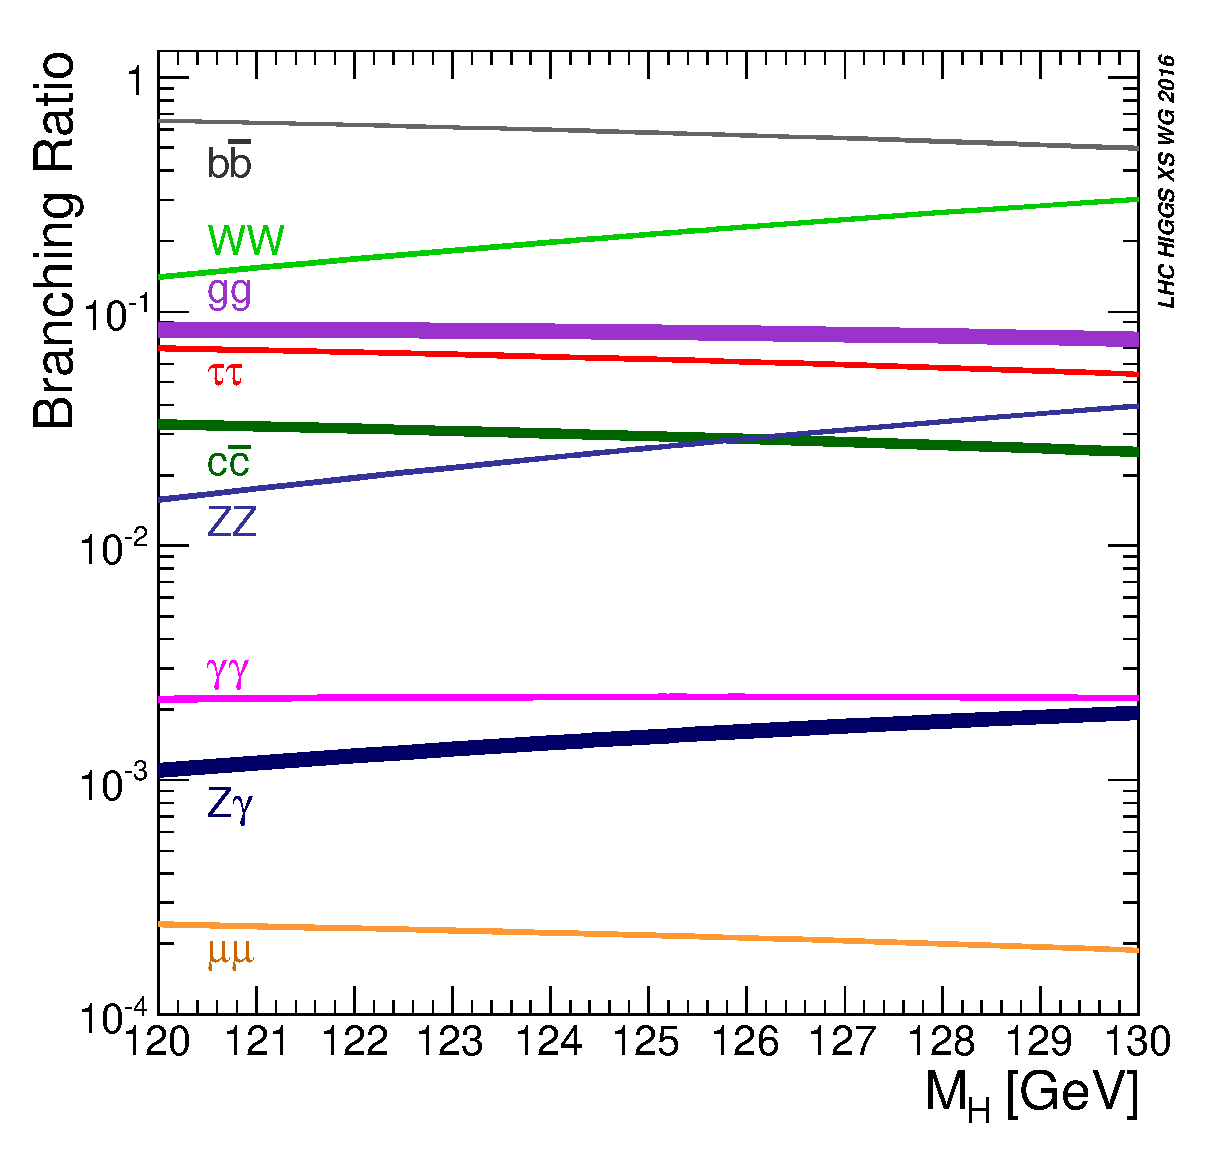
\includegraphics[width=0.5\linewidth]{figures/higgs/higgs_decay_plot.eps}
    \caption{Branching ratios for the decay of the SM Higgs boson near $m_{H} = 125$GeV including theoretical uncertainty bands \cite{PDG2018:Ch11}}
    \label{fig:higgs_decay_plot}
  \end{center}
\end{figure}



\section{Discovery} \label{sec:higgs:discovery}

\section{Boosted Higgs} \label{sec:higgs:boosted}

